\documentclass{article}
\usepackage[utf8]{inputenc}
\usepackage[english]{babel}
\usepackage{graphicx}
\usepackage{amsmath}
\graphicspath{ {images/} }

\begin{document}
% Title page
\begin{titlepage}
    \vspace*{\stretch{1.0}}
    \begin{center}
        \Large{Udacity Machine Learning Nanodegree Capstone}\\
        \LARGE\textbf{Quora Duplicate Question Detection}\\
        \vspace{1cm}
        \large\textit{Raahul Seshadri}\\
        \normalsize{April, 2017}
    \end{center}
    \vspace*{\stretch{2.0}}
\end{titlepage}

% Table of contents
\tableofcontents
\newpage

% Begin sections
\section{Definition}

\subsection{Project Overview}
Websites like Quora\footnote{https://www.quora.com}, StackExchange\footnote{https://stackexchange.com} network (includes the popular programming website StackOverflow\footnote{https://stackoverflow.com}) allow the users to post questions, and the entire community can answer those questions. Ideally, every unique question should be present just once in the system, so that every answer to those questions are present at once place.

However, users are prone to posting duplicate questions, because not all of them check if the question they're asking has already been asked by someone else. This necessitates having an automated duplicate question checker that can check if a question is a duplicate. Whenever the user tries to post a new question, the system can suggest an existing one for perusal.

This project was inspired by Quora's Kaggle challenge\footnote{https://www.kaggle.com/c/quora-question-pairs}. A dataset of question pairs, manually tagged as duplicate or not by human reviewers, has been provided\footnote{https://www.kaggle.com/c/quora-question-pairs} by Quora to train on.

\subsection{Problem Statement}

The problem can be stated as follows:

\begin{center}
\textbf{Given a pair of question texts, detect if they are duplicate or not.}
\end{center}
For example, given the following two questions:

\begin{center}
\textit{Q1: What is the average salary in India?}\\
\textit{Q2: What is the average salary in the United States?}
\end{center}
The system could flag them as either duplicates or not-duplicates. The steps to achieving our duplicate detector are as follows:

\begin{enumerate}
\item{Download and pre-process the Quora training dataset}
\item{Split the Quora training dataset into 90\% training and 10\% test set.}
\item{In the 90\% training set, further 10\% will be used as a validation set.}
\item{Extract usable features from the dataset.}
\item{Train a binary classifier to differentiate between duplicates/non-duplicates.}
\item{Provide a command-line interface so that users can check for duplicates from Quora's test set, or provide his own questions.}
\end{enumerate}

\subsection{Metrics}

Being a binary classification problem, the metric is going to be accuracy:

$$\text{accuracy} = \frac{\text{true positives} + \text{true negatives}}{\text{total samples}}$$
This accuracy will be measured on the test set (10\% of the total dataset).

\begin{enumerate}
\item{\textbf{False negatives}, where a duplicate pair is not detected as such, will lead to degraded user experiences. However, it is also rather harmless, since no information is lost. There is still an opportunity to manually flag them as duplicates, or build such a feature on the platform that is using the duplicate detector.}
\item{\textbf{False positives}, where a question pair that's not a duplicate, but is marked as such, is more dangerous. It can lead to very degraded user experience, since it directly hinders the user trying to perform an action. It is better for the system to err on the side of false negatives than false positives.}
\end{enumerate}

\newpage
\section{Analysis}

\subsection{Data Exploration}

Below is the head (first 20 entries) of the Quora dataset:

\noindent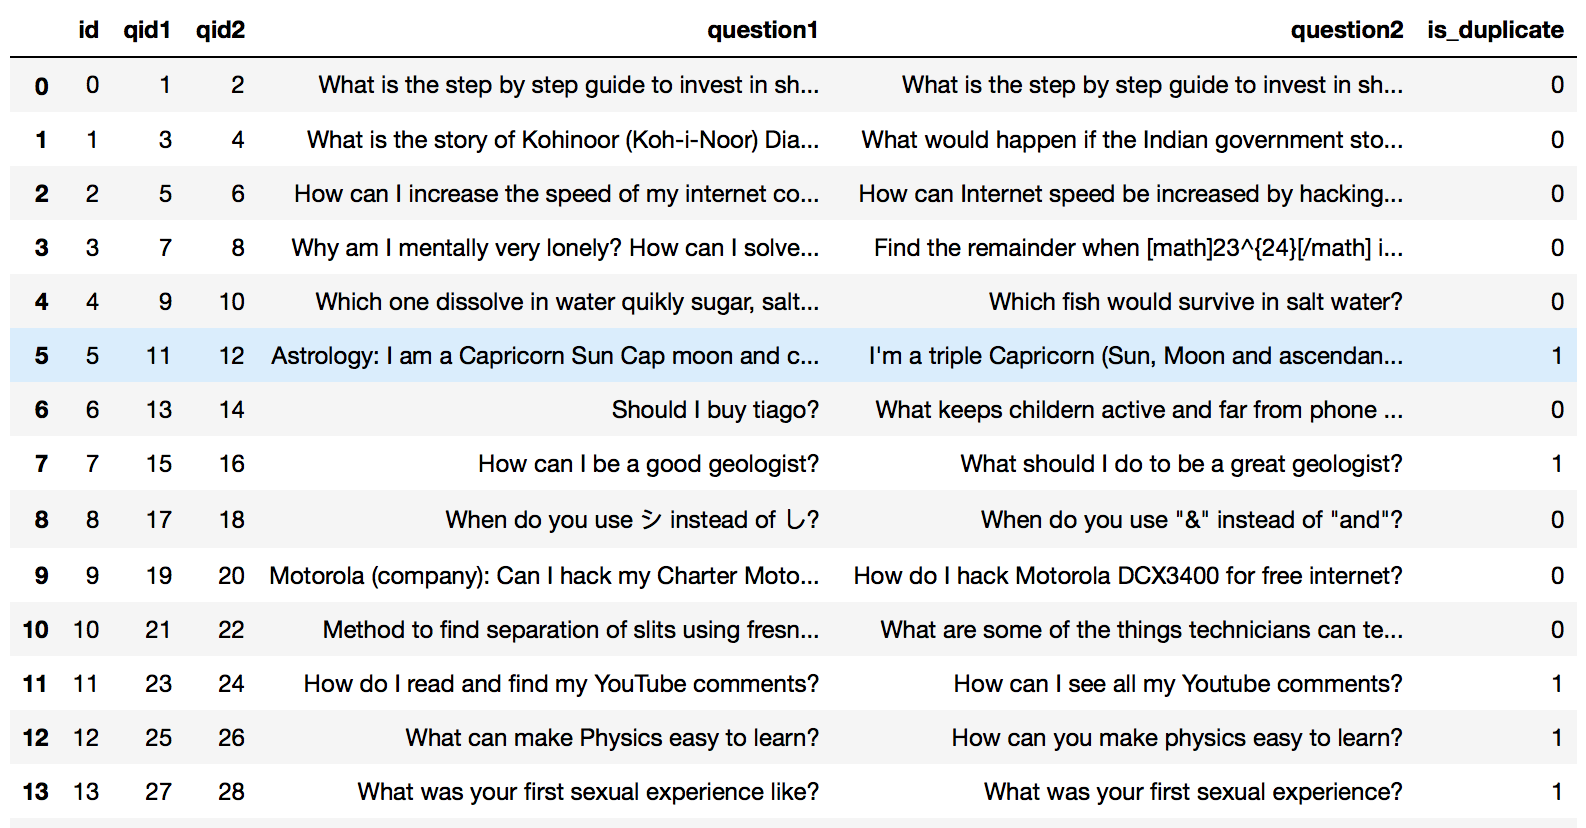
\includegraphics[width=\textwidth]{data_head}
The columns correspond to the following features:

\begin{enumerate}
\item{\textbf{id:} ID to identify the question pair uniquely}
\item{\textbf{qid1:} ID of the first question in the question pair}
\item{\textbf{qid2:} ID of the second question in the question pair}
\item{\textbf{question1:} Text of the first question in the question pair}
\item{\textbf{question2:} Text of the second question in the question pair}
\item{\textbf{is\_duplicate:} Quora reviewer's decision on whether the question pair is duplicate (1) or not (0)}
\end{enumerate}

\subsubsection{Why do we have question IDs for each pair?}
There are two columns of interest, "qid1" and "qid2" that are of interest. The algorithm that we're going to design will only tell us if a given pair of question is a duplicate. However, given a question, we'd also like to find out all the duplicates of it in the system.

For example, if question "1" is a duplicate of question "2", and question "2" is a duplicate of "3", then a system should also know that "1" and "3" are duplicates. Data structures like "union find" allow us to do that. However, this is not in scope of the algorithm that we'll design, but the responsibility of the higher system that will use this duplicate detector.

Which is why the question IDs won't be used as a feature for the duplicate detector, but is still important for the system using the duplicate detector.

\end{document}
